\section{Proceso de Cinemática} \label{sec:proceso_cinematica}


La cinemática de un manipulador robótico comprende el estudio del movimiento de sus eslabones sin considerar las fuerzas involucradas. En este trabajo, se abordan los tres tipos principales de análisis cinemático: directo, diferencial e inverso, utilizando un modelo basado en la convención de Denavit-Hartenberg (DH).

\textbf{Cinemática Directa:} Se establecen la orientación y posición inicial del efector final a través de una matriz de transformación homogénea construida a partir de ángulos de Euler. Utilizando los parámetros DH del archivo \texttt{robot2.csv}, se crea una estructura cinemática del robot que permite calcular la pose del efector final dado un conjunto de posiciones articulares. Además, se generan trayectorias cíclicas articulares (posición, velocidad y aceleración) con un periodo definido, que sirven como base para el análisis cinemático y dinámico.

\textbf{Cinemática Diferencial:} A partir de las trayectorias articulares calculadas, se obtiene la evolución temporal de la posición y orientación del efector final. Se implementa el cálculo del Jacobiano geométrico del robot para obtener la velocidad lineal y angular del efector. Asimismo, se calcula la aceleración utilizando la derivada temporal del Jacobiano, aplicando diferencias finitas. Este análisis permite conocer el comportamiento cinemático instantáneo del robot en cada instante de la trayectoria.

\textbf{Cinemática Inversa:} Se plantea el problema de encontrar las configuraciones articulares necesarias para que el efector final siga una trayectoria deseada en el espacio cartesiano. Se resuelve utilizando un algoritmo iterativo basado en el Jacobiano, el cual converge con alta precisión tras varias iteraciones. Se registran los errores finales y la cantidad de iteraciones requeridas, demostrando la efectividad del método.

En conjunto, estos análisis permiten simular, controlar y validar el comportamiento cinemático completo del manipulador robótico, desde las entradas articulares hasta la ejecución precisa de trayectorias en el espacio.

\newpage
\subsection{Cinemática Directa}

\begin{figure} [h]
	\centering
	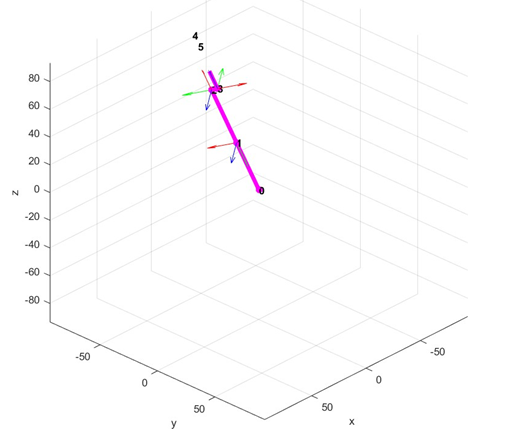
\includegraphics[width=0.7\linewidth]{img/robotcindir}
	\caption{Robot Cinematica Directa}
	\label{fig:robotcindir}
\end{figure}

En esta sección se describe el procedimiento para definir la orientación inicial del efector final del robot, construir la matriz de transformación homogénea de referencia y calcular las trayectorias articulares de forma cíclica.

\subsection*{3.2.1.1. Definición de orientación inicial}

Se definen los ángulos de orientación del efector final respecto a los tres ejes cartesianos:

\begin{verbatim}
	phi = 10;    % Rotación sobre el eje X
	theta = 20;  % Rotación sobre el eje Y
	psi = 30;    % Rotación sobre el eje Z
\end{verbatim}

Estos ángulos, dados en grados, se convierten a radianes y se almacenan como un vector columna:

\begin{verbatim}
	orientacion_inicial = deg2rad([phi; theta; psi]);
	secuencia = "XYZ";
\end{verbatim}

La variable \texttt{secuencia} define el orden de aplicación de las rotaciones según el sistema de ángulos de Euler. En este caso, la secuencia "XYZ" indica que las rotaciones se aplican primero sobre \(X\), luego \(Y\) y finalmente sobre \(Z\).

\subsection*{3.2.1.2. Construcción de la matriz de transformación homogénea inicial}

Se calcula la matriz de rotación utilizando la función \texttt{euler2rotMat} a partir de los ángulos definidos:

\begin{verbatim}
	R = euler2rotMat(orientacion_inicial, secuencia);
\end{verbatim}

Luego, se construye la matriz de transformación homogénea \( A_0 \), que representa la orientación y posición inicial del efector final en el espacio:

\begin{verbatim}
	A0 = [R          posicion_inicial
	zeros(1,3) 1];
\end{verbatim}

\begin{itemize}
	\item \texttt{R}: matriz de rotación \(3 \times 3\)
	\item \texttt{posicion\_inicial}: vector columna \(3 \times 1\) con la posición inicial
	\item \texttt{A0}: matriz homogénea \(4 \times 4\) que define la pose inicial del robot
\end{itemize}

\subsection*{3.2.1.3. Definición del intervalo de tiempo}

Se define un intervalo temporal de 8 segundos con un paso de muestreo de 0.05 s, útil para simular trayectorias continuas:

\begin{verbatim}
	t_inicial = 0;
	t_final = 8;
	t_paso = 0.05;
	t = t_inicial:t_paso:t_final;
\end{verbatim}

\subsection*{3.2.1.4. Lectura de parámetros DH y creación de la estructura del robot}

La estructura cinemática del robot se genera a partir de los parámetros DH almacenados en un archivo CSV:

\begin{verbatim}
	dh = readtable('datos\tabla_DH\robot2.csv');
	robot = crear_robot(dh, A0);
\end{verbatim}

\subsection*{3.2.1.5. Generación de trayectorias articulares}

Finalmente, se genera una trayectoria periódica para los valores articulares \( q \), sus derivadas \( \dot{q} \) (velocidades) y \( \ddot{q} \) (aceleraciones), usando una función cíclica con un periodo de 2 segundos:

\begin{verbatim}
	periodo = 2;    % Periodo del movimiento cíclico
	[q,dq,ddq] = trayectoria_q(robot, t, periodo);
\end{verbatim}

Estas trayectorias se emplean posteriormente para simular el comportamiento dinámico del robot y calcular su cinemática diferencial.


\subsection{Cinemática Diferencial}
Para analizar la cinemática directa del robot, se parte de una tabla de parámetros de Denavit-Hartenberg (DH), la cual contiene la descripción geométrica del manipulador. El archivo \texttt{robot2.csv} contiene los parámetros necesarios para definir cada eslabón del robot: $\theta$, $d$, $a$, y $\alpha$. Estos parámetros son leídos mediante la función \texttt{readtable} y se utiliza una función personalizada \texttt{crear\_robot} que construye el modelo cinemático completo del robot a partir de dicha tabla y una matriz de transformación base $A_0$:

\begin{lstlisting}[language=Matlab]
	dh = readtable('datos\tabla_DH\robot2.csv');
	robot = crear_robot(dh, A0);
\end{lstlisting}

\subsection*{3.2.2.1. Generación de Trayectorias en el Espacio Articular}
Una vez construido el modelo del robot, se generan trayectorias articulares usando perfiles de movimiento cíclico (por ejemplo, funciones senoidales o trapezoidales). El parámetro \texttt{periodo} determina el ciclo del movimiento, y las funciones \texttt{trayectoria\_q} devuelven:

\begin{itemize}
	\item $q(t)$: posición de las articulaciones en función del tiempo,
	\item $\dot{q}(t)$: velocidad articular,
	\item $\ddot{q}(t)$: aceleración articular.
\end{itemize}

Esta información es fundamental para el análisis dinámico del robot, así como para su control. El vector $q(t)$ se puede utilizar como entrada para obtener la pose del efector final mediante la cinemática directa.

\newpage

\subsection{Cinemática Inversa}
\begin{figure} [h]
	\centering
	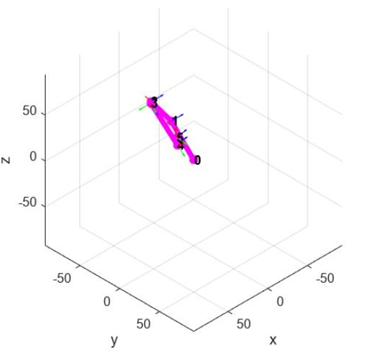
\includegraphics[width=0.7\linewidth]{img/robotcininv}
	\caption{Robot Cinematica Inversa}
	\label{fig:robotcininv}
\end{figure}

\begin{figure} [h]
	\centering
	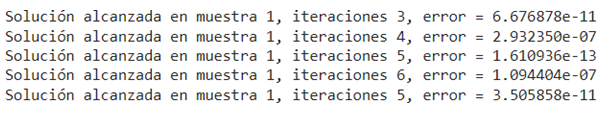
\includegraphics[width=0.7\linewidth]{img/solucionescininv}
	\caption{Soluciones cinematica inversa}
	\label{fig:solucionescininv}
\end{figure}
		
	\textbf{Interpretación:}
	\begin{itemize}
		\item Todos los casos corresponden a la \textbf{muestra 1}, lo que sugiere que se trata de múltiples ejecuciones del algoritmo sobre la misma configuración inicial.
		\item El número de iteraciones varía entre 3 y 6, indicando convergencia rápida en general.
		\item Los errores finales alcanzan valores muy pequeños (del orden de $10^{-11}$ a $10^{-13}$ en algunos casos), lo cual evidencia una alta precisión en la solución encontrada.
		\item Algunos casos presentan errores mayores ($\sim10^{-7}$), lo que puede deberse a condiciones iniciales diferentes, tolerancias del algoritmo o características propias del modelo.
	\end{itemize}
	
	\vspace{0.5cm}
	
	\textbf{Conclusión:}  
	El algoritmo de cinemática inversa utilizado logra encontrar soluciones con alta precisión en un número reducido de iteraciones. Esto sugiere una implementación eficiente y estable, adecuada para aplicaciones de control en tiempo real de robots articulados.
	
